\section{Complex Analysis}

This section introduces the complex-analytic tools needed later for the study of Dirichlet $L$-functions and zeta regularization: holomorphic and meromorphic functions, Cauchy's theorems, power series, analytic continuation, isolated singularities, and residues. The selection follows the treatment of analytic functions, complex integration, Taylor and Laurent series, and residue calculus in Kwok \cite[Chapters 2, 4--6]{Kwok2010}.

\subsection{Holomorphic, Entire, and Meromorphic Functions}

\begin{definition}[Domain]
A domain is a connected open subset of the complex plane $\mathbb{C}$.
\end{definition}

\begin{definition}[Holomorphic function]
Let $D$ be a domain. A function $f:D\to\mathbb{C}$ is holomorphic on $D$ if the complex derivative
\[
 f'(z)=\lim_{h\to 0}\frac{f(z+h)-f(z)}{h}
\]
exists for every $z\in D$.
\end{definition}

\begin{definition}[Entire function]
A function is entire if it is holomorphic on all of $\mathbb{C}$.
\end{definition}

\begin{example}
The functions $f(z)=z^n$ for each nonnegative integer $n$, and $f(z)=e^z$, are entire.
\end{example}

Holomorphicity is a strong condition: a holomorphic function has derivatives of every order and is locally represented by a convergent power series. The Cauchy integral formula below gives a central reason for these properties.

\subsection{Cauchy's Theorem and Integral Formula}

\begin{theorem}[Cauchy--Goursat theorem]
If $f$ is holomorphic on a domain containing a positively oriented simple closed contour $C$ and its interior, then
\[
 \oint_C f(z)\,dz=0.
\]
\end{theorem}

\begin{theorem}[Cauchy integral formula]
Let $C$ be a positively oriented simple closed contour, and suppose that $f$ is holomorphic on and inside $C$. For every point $a$ inside $C$,
\[
 f(a)=\frac{1}{2\pi i}\oint_C\frac{f(z)}{z-a}\,dz.
\]
Moreover, for every integer $n\geq 0$,
\[
 f^{(n)}(a)=\frac{n!}{2\pi i}\oint_C\frac{f(z)}{(z-a)^{n+1}}\,dz.
\]
\end{theorem}

\begin{figure}[H]
\centering
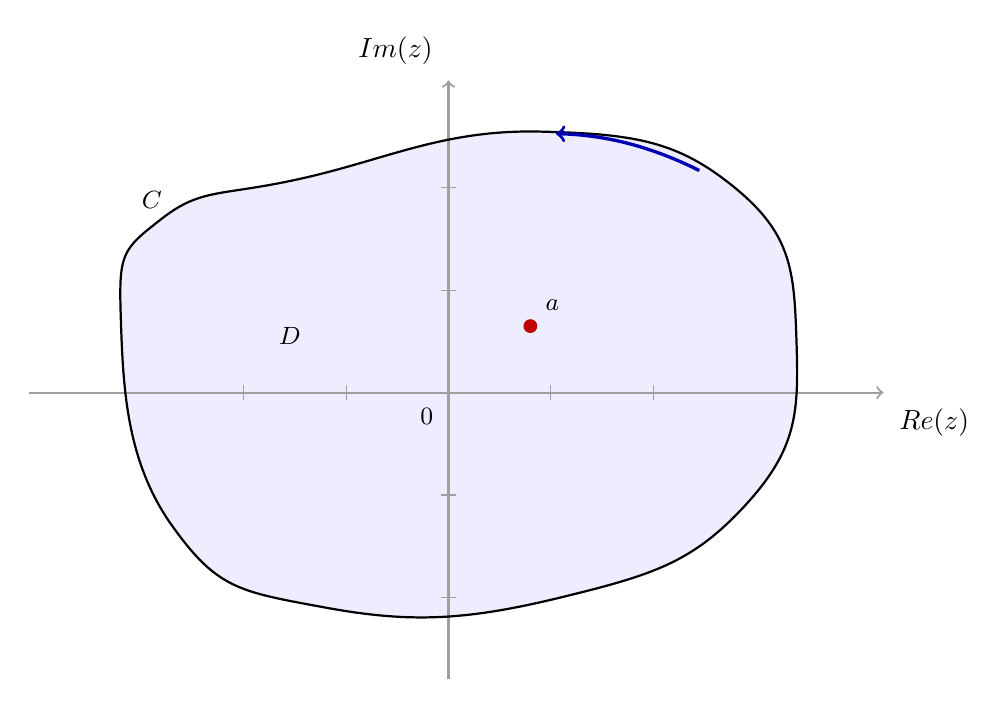
\begin{tikzpicture}[x=1.3cm,y=1.3cm]
    \path[fill=blue!7]
        plot[smooth cycle,tension=0.8] coordinates {
            (-3.2,0.7) (-2.7,-1.3) (-1.2,-2.1) (1.1,-2.0)
            (2.9,-1.1) (3.4,0.5) (2.8,2.0) (0.9,2.55)
            (-1.4,2.1) (-2.8,1.7)
        };
    \draw[->,gray!75,thick] (-4.1,0) -- (4.25,0)
        node[below right=2pt,black] {$\operatorname{Re}(z)$};
    \draw[->,gray!75,thick] (0,-2.8) -- (0,3.05)
        node[above left=2pt,black] {$\operatorname{Im}(z)$};
    \foreach \x in {-2,-1,1,2} {
        \draw[gray!75] (\x,0.07) -- (\x,-0.07);
    }
    \foreach \y in {-2,-1,1,2} {
        \draw[gray!75] (0.07,\y) -- (-0.07,\y);
    }
    \node[below left=2pt,font=\small] at (0,0) {$0$};
    \draw[thick]
        plot[smooth cycle,tension=0.8] coordinates {
            (-3.2,0.7) (-2.7,-1.3) (-1.2,-2.1) (1.1,-2.0)
            (2.9,-1.1) (3.4,0.5) (2.8,2.0) (0.9,2.55)
            (-1.4,2.1) (-2.8,1.7)
        };
    \draw[->,very thick,blue!70!black]
        (2.45,2.17) .. controls (1.95,2.42) and (1.5,2.52) .. (1.05,2.53);
    \node[above left=2pt,font=\small] at (-2.65,1.65) {$C$};
    \node[font=\small] at (-1.55,0.55) {$D$};
    \fill[red!75!black] (0.8,0.65) circle (2.5pt);
    \node[above right=2pt,font=\small] at (0.8,0.65) {$a$};
\end{tikzpicture}
\caption{A positively oriented simple closed contour $C$ enclosing the domain $D$ and the point $a$ in the complex plane.}
\label{fig:cauchy-contour-theorems}
\end{figure}

\begin{corollary}[Taylor expansion]
If $f$ is holomorphic on a disk centered at $a$, then in that disk it has the expansion
\[
 f(z)=\sum_{n=0}^{\infty}\frac{f^{(n)}(a)}{n!}(z-a)^n.
\]
\end{corollary}

\subsection{Taylor and Laurent Series}

Taylor series describe holomorphic functions near ordinary points. When a point is excluded from the domain, a series with both positive and negative powers is needed.

\begin{theorem}[Laurent expansion]
If $f$ is holomorphic on an annulus $r<|z-a|<R$, then there is a unique series
\[
 f(z)=\sum_{n=-\infty}^{\infty}c_n(z-a)^n
\]
that converges to $f$ throughout the annulus, uniformly on every compact subannulus. Its coefficients are
\[
 c_n=\frac{1}{2\pi i}\oint_{|z-a|=\rho}
 \frac{f(z)}{(z-a)^{n+1}}\,dz,
 \qquad r<\rho<R.
\]
\end{theorem}

The coefficient $c_{-1}$ is called the residue of $f$ at $a$, denoted by $\operatorname{Res}(f,a)$.

\subsection{Isolated Singularities and Residues}

\begin{definition}[Isolated singularity]
A point $a$ is an isolated singularity of $f$ if $f$ is holomorphic in some deleted neighborhood $0<|z-a|<r$ of $a$.
\end{definition}

The Laurent expansion classifies isolated singularities:
\begin{itemize}
    \item The singularity is removable if all coefficients with negative index vanish.
    \item It is a pole of order $m$ if $c_{-m}\neq 0$ and $c_n=0$ for every $n<-m$.
    \item It is essential if infinitely many coefficients with negative index are nonzero.
\end{itemize}

\begin{figure}[H]
\centering
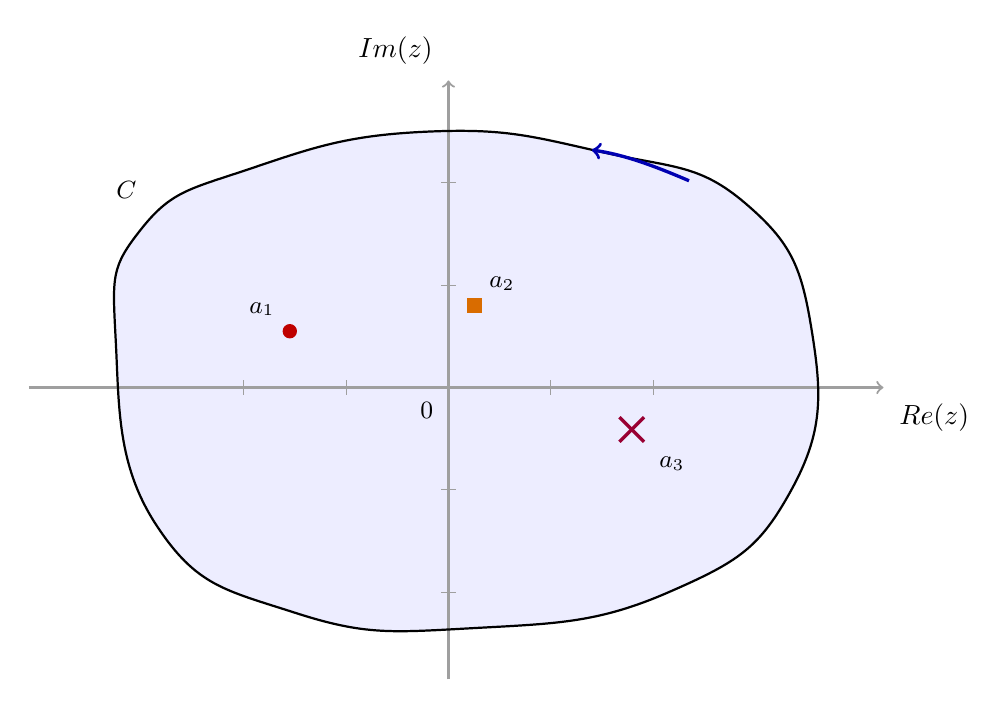
\begin{tikzpicture}[x=1.3cm,y=1.3cm]
    \path[fill=blue!7]
        plot[smooth cycle,tension=0.8] coordinates {
            (-3.25,0.45) (-2.85,-1.35) (-1.5,-2.2) (0.25,-2.35)
            (2.15,-2.0) (3.35,-1.0) (3.55,0.55) (2.9,1.8)
            (1.5,2.3) (-0.2,2.5) (-1.9,2.15) (-3.0,1.55)
        };
    \draw[->,gray!75,thick] (-4.1,0) -- (4.25,0)
        node[below right=2pt,black] {$\operatorname{Re}(z)$};
    \draw[->,gray!75,thick] (0,-2.85) -- (0,3.0)
        node[above left=2pt,black] {$\operatorname{Im}(z)$};
    \foreach \x in {-2,-1,1,2} {
        \draw[gray!75] (\x,0.07) -- (\x,-0.07);
    }
    \foreach \y in {-2,-1,1,2} {
        \draw[gray!75] (0.07,\y) -- (-0.07,\y);
    }
    \node[below left=2pt,font=\small] at (0,0) {$0$};
    \draw[thick]
        plot[smooth cycle,tension=0.8] coordinates {
            (-3.25,0.45) (-2.85,-1.35) (-1.5,-2.2) (0.25,-2.35)
            (2.15,-2.0) (3.35,-1.0) (3.55,0.55) (2.9,1.8)
            (1.5,2.3) (-0.2,2.5) (-1.9,2.15) (-3.0,1.55)
        };
    \draw[->,very thick,blue!70!black]
        (2.35,2.02) .. controls (2.0,2.17) and (1.7,2.28) .. (1.4,2.32);
    \node[above left=2pt,font=\small] at (-2.9,1.7) {$C$};

    \fill[red!75!black] (-1.55,0.55) circle (2.6pt);
    \node[above left=2pt,font=\small] at (-1.55,0.55) {$a_1$};
    \node[draw=orange!85!black,fill=orange!85!black,minimum size=5pt,inner sep=0pt]
        at (0.25,0.8) {};
    \node[above right=2pt,font=\small] at (0.25,0.8) {$a_2$};
    \draw[purple!80!black,line width=1.2pt] (1.67,-0.53) -- (1.91,-0.29);
    \draw[purple!80!black,line width=1.2pt] (1.67,-0.29) -- (1.91,-0.53);
    \node[below right=2pt,font=\small] at (1.91,-0.53) {$a_3$};
\end{tikzpicture}
\caption{The counterclockwise contour $C$ encloses isolated singularities: a simple pole at $a_1$ (circle), a pole of order two at $a_2$ (square), and an essential singularity at $a_3$ (cross).}
\label{fig:isolated-singularities-contour}
\end{figure}

\begin{definition}[Meromorphic function]
A function on a domain is meromorphic if it is holomorphic there except at isolated poles.
\end{definition}

\begin{example}
At $z=0$, the function $\sin z/z$ has a removable singularity, $1/z^2$ has a pole of order two, and $e^{1/z}$ has an essential singularity. These classifications follow from their Laurent expansions at the origin.
\end{example}

\begin{theorem}[Residue theorem]
Let $C$ be a positively oriented simple closed contour, and let $f$ be holomorphic on and inside $C$ except at finitely many isolated singularities $a_1,\ldots,a_k$ in its interior. Then
\[
 \oint_C f(z)\,dz=2\pi i\sum_{j=1}^{k}\operatorname{Res}(f,a_j).
\]
\end{theorem}

\begin{proof}
Remove small, disjoint disks around the singularities. The function is holomorphic on the remaining region, so Cauchy's theorem equates the integral over $C$ with the sum of the integrals over the small, positively oriented circles around each $a_j$. Integrating the Laurent series around each circle leaves only its $(z-a_j)^{-1}$ term, whose integral is $2\pi i\operatorname{Res}(f,a_j)$.
\end{proof}

\begin{example}
The Laurent expansion at $z=0$ is
\[
 \frac{e^z}{z^2}=\frac{1}{z^2}+\frac{1}{z}+\frac{1}{2!}+\cdots,
\]
so $\operatorname{Res}(e^z/z^2,0)=1$. Therefore, for any positively oriented circle centered at the origin,
\[
 \oint_C\frac{e^z}{z^2}\,dz=2\pi i.
\]
\end{example}

\subsection{Analytic Continuation}

\begin{definition}[Analytic continuation]
Let $f$ be holomorphic on a domain $D$. A holomorphic function $F$ on a larger domain $D'\supset D$ is an analytic continuation of $f$ if $F(z)=f(z)$ for every $z\in D$. If $F$ is meromorphic on $D'$, it is called a meromorphic continuation.
\end{definition}

\begin{theorem}[Identity theorem]
If two holomorphic functions on a connected domain agree on a set with a limit point in that domain, then they agree everywhere on the domain.
\end{theorem}

The identity theorem ensures that an analytic continuation, when it exists, is unique on a connected domain. For example, the geometric series
\[
 \sum_{n=0}^{\infty}z^n=\frac{1}{1-z},\qquad |z|<1,
\]
has the analytic continuation $1/(1-z)$ to $\mathbb{C}\setminus\{1\}$. These ideas will be used later when studying the continuation and singularities of zeta and Dirichlet $L$-functions.